\chapter{Results}

\section{Static and dynamic difference}

\begin{figure}[h!]
\begin{subfigure}[b]{0.5\textwidth}
    \centering
    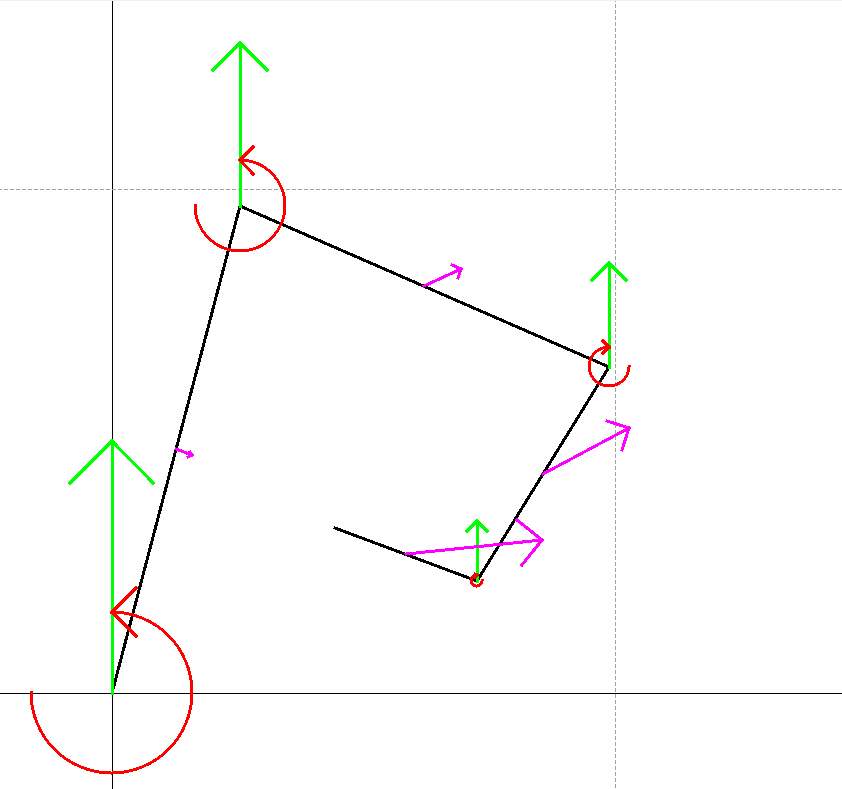
\includegraphics[width=\linewidth]{result2_static}
    \caption{Without dynamic effects}
    \label{result_static}
\end{subfigure}
\hfill
\begin{subfigure}[b]{0.5\textwidth}
    \centering
    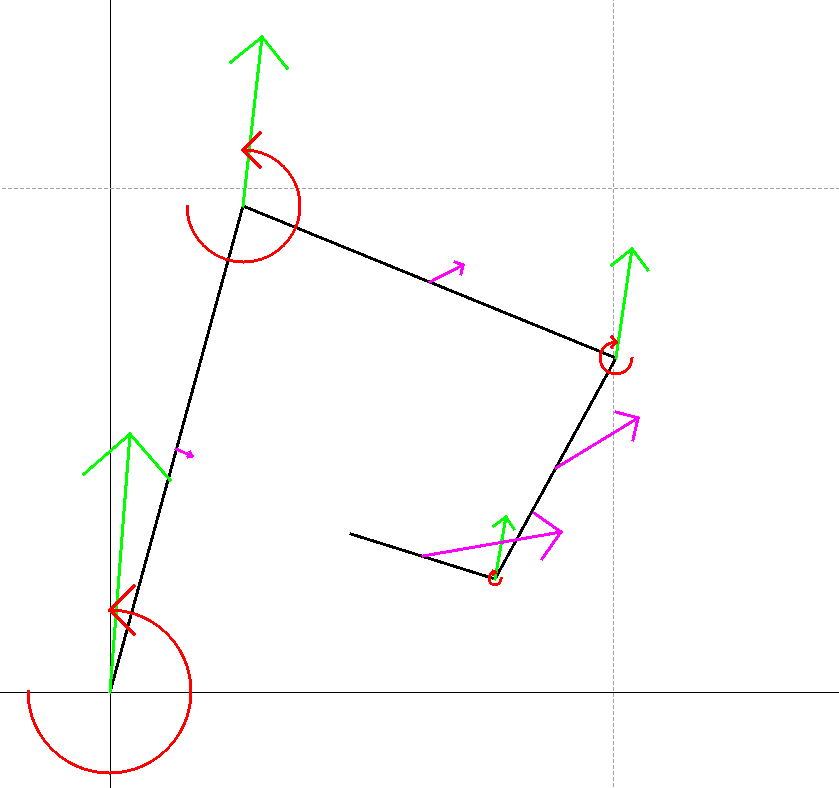
\includegraphics[width=\linewidth]{result2_dynamic}
    \caption{With dynamic effects}
\end{subfigure}
\caption{Comparison of force response in system without and with dynamic effects}
\label{result_img}
\end{figure}

\figref{result_img} shows a robot configuration halfway through an animation where the dynamic contribution is (a) turned off and (b) turned on. Since no inertial forces are considered in \figref{result_static} it is expected that this would produce results similar to a static case. The acceleration in magenta are the same in both figures but some differences in force and torque can be seen.

Firstly, in the static case the joint forces only contain a vertical component. This is as expected as the resulting joint force should be a result of gravity forces only. When considering inertial forces in (b) it is clear that they now have a horizontal component. This is coherent with the acceleration that can be seen. In this situation the joint forces has to support the change in momentum in addition to the weight of the link.

\section{Convergence}

The addition to the joint force because of inertial forces are directly related to the acceleration of the links,  \eqref{linear_equi} and (\ref{linear_mom}). The following section will present the results from a test which intention was to verify that as the acceleration got slower, the forces would converge to those of a static case.

\figref{results} shows the force magnitude as function of animation percentage for multiple animation lengths. The used animation is described in \figref{animation}. It can be seen that the inertial forces have a big impact on the force magnitude for rapid movement and that the force converges to the static case as the animation time is increased.


\begin{figure}[h!]
    \centering
    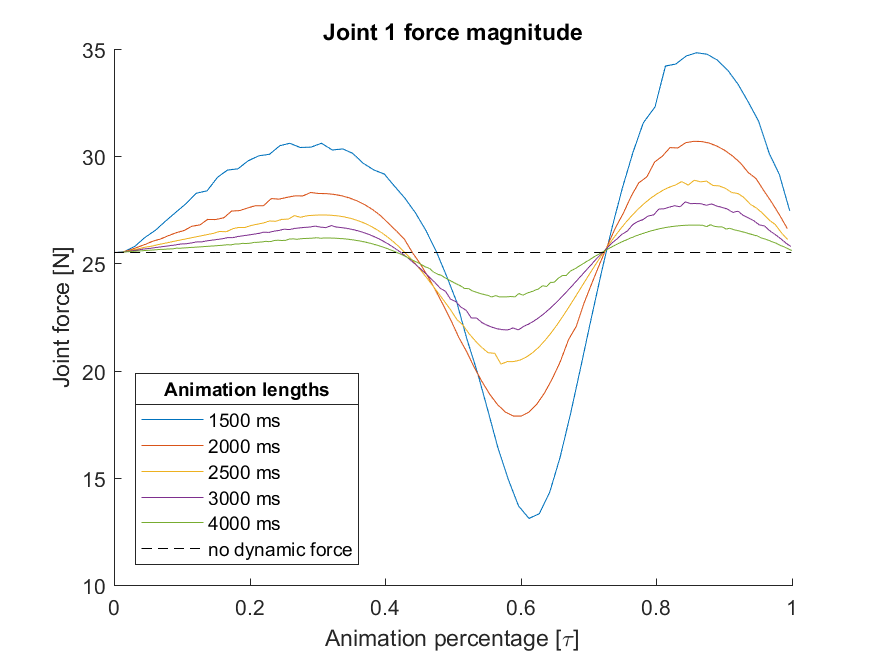
\includegraphics[width=.9\textwidth]{joint_force_comp}
    \caption{Joint force magnitude for multiple animation times}
    \label{results}
\end{figure}